%%--------- Comandos especiales
\newcommand{\vecr}{\mathbf{r}}
\newcommand{\veck}{\mathbf{k}}
\newcommand{\nnet}{N_{\theta}(\mathbf{r})}
%%
\chapter{Neural networks as an approximation for the bridge function} % Main chapter title

\label{Cap3} % Change X to a consecutive number; for referencing this chapter elsewhere, use \ref{ChapterX}

%----------------------------------------------------------------------------------------
%	SECTION 1
%----------------------------------------------------------------------------------------

Neural networks can be used as \emph{universal approximators}~\cite{hornikMultilayerFeedforwardNetworks1989, hornikApproximationCapabilitiesMultilayer1991, cybenkoApproximationSuperpositionsSigmoidal1989},
in other words, they can take the form of any continuous function for some specific
types of architectures.
In particular, it is hypothesized that a neural network might be useful as a bridge function
parametrization in the closure expression for the Ornstein-Zernike equation. If this is true,
then choosing a particular approximation can be avoided for a given interaction potential, 
and leave the choice of the bridge function to the neural network itself, while
simultaneously solving the Ornstein-Zernike equation.

In this chapter, we show in detail the methodology created to achieve such a task, and
the mathematical structure with which a neural network can be used to solve the
Ornstein-Zernike equation.
These results are compared to those obtained from computer simulations to assess the
quality of the solution.
In the appendix, the detailed algorithm used to solve the Ornstein-Zernike equation
is presented, along with a detailed computation of the gradients used for the
training scheme. Here, we shall focus only on the main results and the algorithm structure
in general.

\section{Parametrization of the bridge function}

The Ornstein-Zernike equation is given by the following expression

\begin{subequations}
    \begin{align*}
         & c(\vecr) = h(\vecr) +
        n \int_{V}
        c(\vecr^{\prime})
        h(\lvert \vecr - \vecr^{\prime} \rvert)
        d\vecr^{\prime} \label{eq:oz1} \\
         & c(\vecr)
        = \exp{\left[
                -  \beta u(\vecr)
                +  \gamma(\vecr)
                + B(\vecr)
                \right]} -
        \gamma(\vecr)
        - 1
    \end{align*}
\end{subequations}

with the already known notation for each quantity (Ref a marco teórico).

Let $\nnet$ be a neural network with weights $\theta$. The main hypothesis
of this chapter is that $\nnet$ can replace the bridge function $B(\vecr)$
in the previous equation, which will yield the following expression for
the closure relation

\begin{equation}
    c(\vecr) = \exp{\left[
            -  \beta u(\vecr)
            +  \gamma(\vecr)
            + \nnet
            \right]} -
    \gamma(\vecr)
    - 1 .
    \label{eq:parametrizacion}
\end{equation}

With this new expression, the main problem to solve is to find the weights
of $\nnet$ that can successfully solve the Ornstein-Zernike equation
for a given interaction potential, $\beta u(\vecr)$.

%----------------------------------------------------------------------------------------
%	SECTION 2
%----------------------------------------------------------------------------------------

\section{Training scheme}
Now that a parametrization is defined, a way to fit the weights of the neural network must
be devised. This new numerical scheme must also be able to solve the OZ equation, while
simultaneously finding the appropiate weights for $\nnet$.

\subsection{Cost function}
It was mentioned previously that the main problem to solve is to find the weights of
$\nnet$ that can successfully solve the Ornstein-Zernike equation
for a given interaction potential.
To solve such problem, a \textbf{cost function} must be defined, and be used as part of
a \emph{minimization} problem.

To define such a function, we consider the successive approximations obtained from the
iterative Piccard scheme to solve the OZ equation, $\{\gamma_1(\vecr), \gamma_2(\vecr), \dots, \gamma_n(\vecr)\}$.
From this, we expect to have found a solution when each approximation
is \emph{close enough} to the previous one. This can be translated into the following
cost function

\begin{equation}
    J(\theta) = \left[\gamma_{n}(\vecr; \theta) - \gamma_{n-1}(\vecr; \theta) \right]^2
    \label{eq:costo}
\end{equation}

where $\gamma_{n}(\vecr; \theta)$ is the $n-$th approximation of the indirect
correlation function, $\gamma(\vecr)$.
The notation $\gamma(\vecr; \theta)$ indicates that the function depends implicitly
on the weights of the neural network, as seen in equation~\eqref{eq:parametrizacion}.
This means that, if the weights of $\nnet$ change, we should expect a change in the output
from the $\gamma$ function. Nevertheless, this does not mean that the indirect
correlation function itself depends explicitly, nor directly, on the weights of
$\nnet$.

In other words, the expression~\eqref{eq:costo} is requiring for the last two approximations
to be as equal as possible. This will enforce a change on the weights every time both
approximations deviate between them.

\subsection{Optimization problem}
With a cost function at hand, an optimization problem can be defined such that the
weights of $\nnet$ will be adjusted properly.

This optimization problem is in fact an \emph{unconstrained optimization problem},
and it is defined simply as

\begin{equation}
    \begin{aligned}
         & \underset{\theta}{\text{min}}
         & & J(\theta)
    \end{aligned}
    .
    \label{eq:optimizacion}
\end{equation}

This formulation is just a search for the best values for the weights that minimize
the squared difference between successive approximations.
This optimization problem can be solved iteratively, along with the solution of the
OZ equation, which is also an iterative process.

\subsection{Weight updates}
The iterative method employed to adjust the weights of $\nnet$ is based on the
\emph{gradient descent} method~\cite{nocedalNumericalOptimization2006}.
The most general update rule for a method based on gradient descent reads

\begin{equation}
    \theta_{n+1} = \theta_n - \eta \nabla_{\theta} J(\theta) .
    \label{eq:gradiente}
\end{equation}

where $\eta$ is known as the \emph{learning rate}, and it is a hyperparameter
that controls the step size at each iteration while moving toward the minimum
of a cost function. Tthis value needs to be \emph{tuned} accordingly, so
that the method converges properly.

% TODO: Cambiar el nombre del apéndice
Regardless of the particular expression for the weight updates, every method
based on the gradient descent method \emph{requires} the gradient information from
the cost function with respect to the weights, $\nabla_{\theta} J(\theta)$.
In this particular case, the detailed computation of the gradient is described in
the appendix (Ref a apéndice).
Once this information is obtained, all that is left is to build an algorithm that
can correctly use this training scheme and solve the OZ equation.

\subsection{Solving the Ornstein-Zernike equation with neural networks}
Having described all the necessary elements needed, a general layout for the solution
of the Ornstein-Zernike using neural networks is now presented.

Thus, we have the following step to solve the OZ using the parametrization~\eqref{eq:parametrizacion}:

\begin{enumerate}
    \item Given a particular interaction potential $\beta u(\vecr)$, equation~\eqref{eq:parametrizacion} is used to obtain the value of the direct correlation function $c(\vecr; \theta)$, which now depends implicitly on the weights of $\nnet$. In this step, an initial value for $\gamma_{n}(\vecr)$ is needed, which is initialized based on the five-point Ng methodology. (Ref a apéndice)
    \item The newly found function $c(\vecr; \theta)$ is transformed to a reciprocal space by means of the Fourier transform yielding the new function $\hat{c}(\veck; \theta)$.
    \item Then, the full OZ equation(Ref a ec) is Fourier transformed. Using the information from the previous step, a new estimation of the indirect correlation function is obtained, $\hat{\gamma}_{n+1}(\veck; \theta)$.
    \item The Fourier transform is applied once again to return all the functions to real space. With this operation, a new estimation $\gamma_{n+1}(\vecr; \theta)$ is computed from the transformed function, $\hat{\gamma}_{n+1}(\veck; \theta)$.
    \item Both estimations, $\gamma_{n}$ and $\gamma_{n+1}$, are used to evaluate the cost function~\eqref{eq:costo}, and the computation of the gradient $\nabla_{\theta} J(\theta)$ is performed.
    \item The weights $\theta$ are updated with the gradient descent rule~\eqref{eq:gradiente}, and the process is repeated from step 1. In the next iteration, the initial value for the indirect correlation function will be $\gamma_{n+1}$, and a new estimation $\gamma_{n+2}$ will be obtained. This process is repeated until convergence.
\end{enumerate}

\subsection{Convergence criterion}
The procedure describe in the previous section is repeated indefinetely until convergence
is achieved. This convergence criterion is defined as follows

\begin{equation}
    {\lvert \gamma_{n+1} - \gamma_{n} \rvert}^2 \leq \epsilon
    \label{eq:tolerancia}
\end{equation}

where $\lvert \cdot \rvert$ indicates the absolute value, and $\epsilon \in \numlist{0; 1}$.
In particular, the numerical tolerance in all the experiments has a value of $\epsilon = \num{1e-5}$.
This means that the weights are adjusted until the successive estimations of the $\gamma$
functions are equal between them, up to the defined tolerance $\epsilon$.

%----------------------------------------------------------------------------------------
%	SECTION 3
%----------------------------------------------------------------------------------------
\section{Implementation}
In this section we detail the most important aspects about the implementation of the
method described in the previous section. This includes the topology of the neural network,
the optimization method, and the choice of activation function. The physical parameters used
to solve the OZ equation are also outlined.

\subsection{Choice of optimization algorithm}
The general rule for the weight update based on gradient descent~\eqref{eq:gradiente} was
implemented to solve the optimization problem, but numerical instabilities rendered this 
method unstable and convergence was almost never achieved.

To solve this issue, the \emph{Adam}~\cite{kingmaAdamMethodStochastic2017} optimization 
method was then chosen. This optimization method is an excellent choice for the training
of neural networks, even more so when the gradient is expected to be \emph{sparse}, i.e.
most of the elements of the gradient itself are zeroes.
The \emph{Adam} method uses several rules to adjust the descent direction of the gradient,
as well as the hyperparameters related to the acceleration mechanism of the method.
Notably, there are two important hyperparameters used by the method, $\beta_1$,
which controls the moving average of the computed gradient; and $\beta_2$, which controls
the gradient squared. Both parameters are necessary for the optimal convergence of the
algorithm.

The equations that define the optimization method are the following

\begin{align}
    m &= \beta_1 m - (1 - \beta_1) \nabla_{\theta} J(\theta) \nonumber \\
    s &= \beta_2 s + (1 - \beta_2) \nabla_{\theta} J(\theta) \odot \nabla_{\theta} J(\theta) \nonumber \\
    \hat{m} &= \frac{m}{1 - \beta_1^t} \nonumber \\
    \hat{s} &= \frac{s}{1 - \beta_2^t} \nonumber \\
    \theta &= \theta + \eta \hat{m} \oslash \sqrt{\hat{s} + \varepsilon}
    \label{eq:adam}
\end{align}

where $\odot$ is the elementwise multiplication, or Hadamard product; $\oslash$
is the elementwise division, or Hadamard division; and $\varepsilon$ is a smoothing
value to prevent division by zero.

In the results presented in this chapter, the parameters were fixed to the ones reported
as optimal in the original work~\cite{kingmaAdamMethodStochastic2017}, which are
$\beta_1=\num{0.9}$ and $\beta_2=\num{0.999}$. It is important to note that this method
has its own mechanisms to control and modify the gradients, as well as the hyperparameters.
This makes it a \emph{hands-off} method, without the need to tune the hyperparameters.
The \emph{learning rate}, $\eta$ in equation~\eqref{eq:gradiente}, was fixed to
$\eta=\num{1e-4}$ for all the experiments.

\subsection{Neural network architecture}

\begin{figure}[t]
    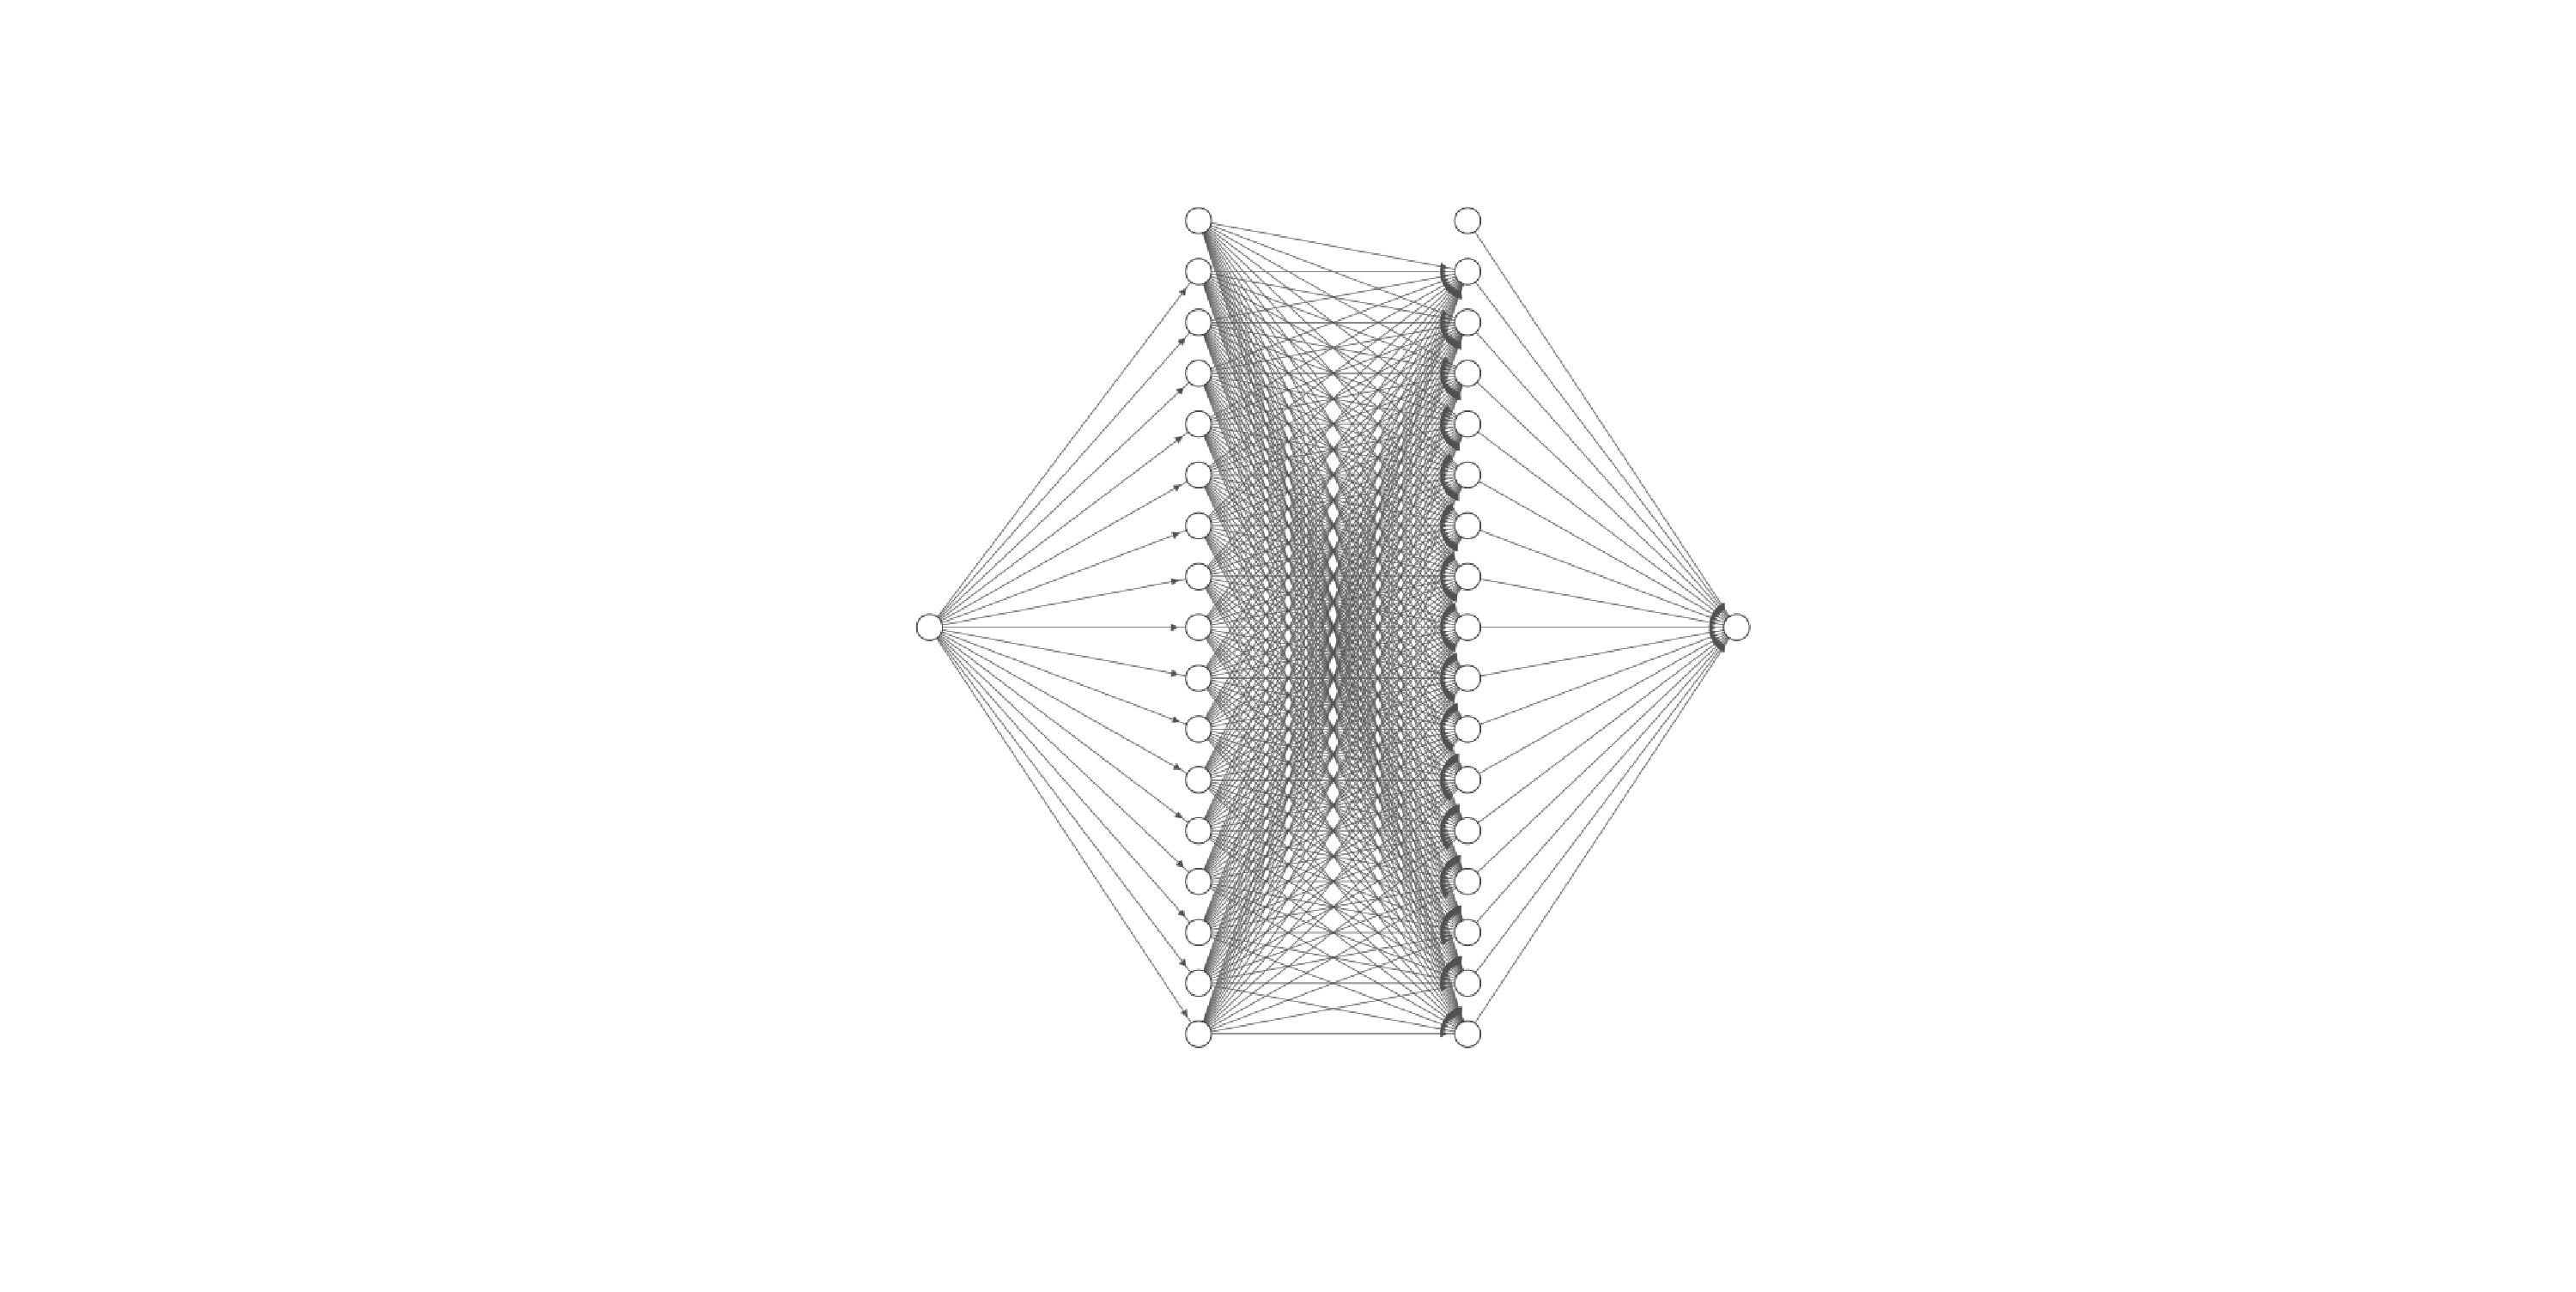
\includegraphics[width=\textwidth]{figuras/capitulo-3/neural-network.pdf}
    \vspace{-1.5cm}
    \caption[General schematics of a neural network.]{Cartoon of a fully connected multilayer neural network. Note that there are two \emph{hidden layers}. The circles represent the \emph{nodes} or \emph{units} used to compute the final output. These nodes are using an activation function to account for nonlinearities. The top-most nodes that seem different from the main nodes are known as the \emph{bias} nodes. The real architecture used in this chapter is larger, with many more nodes and connections, but the topology is the same.}
    \label{fig:nn-esquema}
\end{figure}

The neural network architecture used in all the experiments is very similar to the one
shown in figure~\ref{fig:nn-esquema}, with the exception of the number of nodes in all the
layers.
Particularly, the neural network is made of \emph{four layers}, all connected among them.
There is an \emph{input} layer, two \emph{hidden} layers, and a final \emph{output} layers.
All layers have the same number of nodes, which is 4096. Additional nodes are added to the
final two layers that serve as the \emph{bias}.

All the weights must be initialized appropiately, and in this case the Glorot uniform
distribution was used~\cite{glorotUnderstandingDifficultyTraining2010}, which has proven
to be a way to help the convergence of neural networks. This means that the weights
are initialized as $\theta_{ij} \sim U \left[ -\frac{6}{\sqrt{(in + out)}}, \frac{6}{\sqrt{(in + out)}} \right]$,
where $in$ represents the number of units in the input layer, and $out$ the number of
units in the output layer. All bias nodes were initialized to be zero.

The activation function used was the \emph{ReLU}~\cite{glorotDeepSparseRectifier2011}
function which has the form

\begin{equation*}
    \text{ReLU}(x) = \max{(0, x)} .
\end{equation*}

This activation function is applied to all the nodes in the layers, with the exception
of the input layer. This function was chosen due to the fact that the other most common
functions ($\tanh, \text{softmax}$, etc.) generated numerical instabilities in the
algorithm when training the neural network.

\subsection{Physical parameters}

% TODO: Poner la referencia a la ecuación del potencial
To solve the OZ equation a cutoff radius of $r_c=7\sigma$ was used, where $\sigma$ is the
particle diameter and it fixed to be $\sigma=1$.
The interaction potential used was the pseudo hard sphere potential (Ref a ec.), both
for the solution of the OZ equation as well as the results obtained from computer simulations.

Seven different densities were explored in the range $\phi \in [\num{0.15}, \num{0.45}]$, 
with $\Delta \phi = \num{0.05}$.
For each density value, a grid of 70 points was used to ensure convergence of the iterative
algorithm when solving for the OZ equation. This was not the case of the computer 
simulations, where such partition is not needed.

%----------------------------------------------------------------------------------------
%	SECTION 4
%----------------------------------------------------------------------------------------
\section{Results}

% \begin{figure}[p]
%     \begin{tabular}{cc}
%         \includegraphics[width=0.47\textwidth]{figuras/capitulo-3/sim_p=0.15.pdf} & 
%         \includegraphics[width=0.47\textwidth]{figuras/capitulo-3/comparison_p=0.15.pdf} \\
%         (a) & (b) \\[6pt]
%     \end{tabular}
%     \captionsetup{singlelinecheck=off}
%     \caption[Radial distribution functions with neural networks.]{Radial distribution functions obtained from computer simulations and with the methodology described in this chapter, with the neural network parametrization. Four different density values are presented:
%     \begin{enumerate*}[label=(\alph*),itemjoin={,\enspace}]
%         \item $\phi=\num{0.15}$
%         \item $\phi=\num{0.25}$
%         \item $\phi=\num{0.35}$
%         \item $\phi=\num{0.45}$
%     \end{enumerate*}
%     . In each figure, a comparison between three common bridge function approximation appear along with the computer simulation results and the neural network approximation. The approximations are \emph{mV}, modified Verlet; \emph{PY}, Percus-Yevick; y \emph{HNC}, and Hypernetted Chain.}
%     \label{fig:estructuras-neuronales}
% \end{figure}

\begin{figure}
    \centering
    \includegraphics[width=\textwidth]{figuras/capitulo-3/comparison_p=0.15.pdf}
    \caption[Radial distribution function, $\phi=0.15$.]{The radial distribution function for density value $\phi=0.15$ obtained from computer simulations, and three different approximations:
    \begin{enumerate*}[label=(\alph*),itemjoin={,\enspace}]
        \item \emph{mV}, modified Verlet,
        \item \emph{HNC}, Hypernetted Chain,
        \item \emph{Neural network}, neural network approximation.
    \end{enumerate*}
    }
    \label{fig:rdf15}
\end{figure}

\begin{figure}
    \centering
    \includegraphics[width=\textwidth]{figuras/capitulo-3/comparison_p=0.25.pdf}
    \caption[Radial distribution function, $\phi=0.25$.]{The radial distribution function for density value $\phi=0.25$ obtained from computer simulations, and three different approximations:
    \begin{enumerate*}[label=(\alph*),itemjoin={,\enspace}]
        \item \emph{mV}, modified Verlet,
        \item \emph{HNC}, Hypernetted Chain,
        \item \emph{Neural network}, neural network approximation.
    \end{enumerate*}
    }
    \label{fig:rdf25}
\end{figure}

\begin{figure}
    \centering
    \includegraphics[width=\textwidth]{figuras/capitulo-3/comparison_p=0.35.pdf}
    \caption[Radial distribution function, $\phi=0.35$.]{The radial distribution function for density value $\phi=0.35$ obtained from computer simulations, and three different approximations:
    \begin{enumerate*}[label=(\alph*),itemjoin={,\enspace}]
        \item \emph{mV}, modified Verlet,
        \item \emph{HNC}, Hypernetted Chain,
        \item \emph{Neural network}, neural network approximation.
    \end{enumerate*}
    }
    \label{fig:rdf35}
\end{figure}

\begin{figure}
    \centering
    \includegraphics[width=\textwidth]{figuras/capitulo-3/comparison_p=0.45.pdf}
    \caption[Radial distribution function, $\phi=0.45$.]{The radial distribution function for density value $\phi=0.45$ obtained from computer simulations, and three different approximations:
    \begin{enumerate*}[label=(\alph*),itemjoin={,\enspace}]
        \item \emph{mV}, modified Verlet,
        \item \emph{HNC}, Hypernetted Chain,
        \item \emph{Neural network}, neural network approximation.
    \end{enumerate*}
    }
    \label{fig:rdf45}
\end{figure}

Using all the elements previously described, it is time to investigate the results obtained
from the proposed methodology. The main point of discussion will be the radial distribution
function \textemdash $g(r^*)$ \textemdash for different values of densities, both in the
low and high density regimes.

\subsection{Low densities}
To begin the discussion, this section will deal with the low 
density values $\phi=\numlist{0.15; 0.25}$, which are shown in plots (a) and (b) in 
figure~\ref{fig:rdf45}.
The results show that, at low densities, the HNC and neural network approximations are
more precise than the modified Verlet approximation. Although, all
approximations seem to fall short compared to computer simulations. It is specially
important to note that the neural network approximation is a little bit more precise than
the HNC approximation, which can be qualitatively appraised by observing the estimation of 
the main peak in the radial distribution function. This peak can be found in the vicinity 
of $r^* = \sigma$. Nevertheless, it is still overestimated, which is the same case for the
HNC approximation. However, this is not the case for the Percus-Yevick and modified Verlet 
approximations, which undervalue the main peak.

It is also important to notice the functional form of $g(r^*)$. For the HNC and neural
network approximations, it appears to have the same form between approximations, and it 
might as well be the same. This would imply that, somehow, the weights of the neural network
were updated enough such that a minimum was found, and this minimum was very close to the
HNC approximation. In other words, the results suggest that the weights are very close to
zero, such that when the neural network is evaluated, the output is close to the
result obtained from the HNC approximation.
Another important aspect to observe is that this functional form is slightly different
to the one seen from computer simulations, and that the modified Verlet approximation is 
closer to the form found in the computer simulations results.

\subsection{High densities}
We now turn our discussion to the high density values of $\phi=\numlist{0.35; 0.45}$,
represented in plots (c) and (d) in the figure~\ref{fig:estructuras-neuronales}.
In the same spirit as before with the low densities, the HNC and neural network 
approximations are not precise when compared to computer simulations. In this case,
the Percus-Yevick and modified Verlet are even more precise, which was expected.
This is because the HNC approximation is a very good approximation for long range
interaction potentials (Ref faltante), and Percus-Yevick as well as modified Verlet are 
better suited for short range potentials, such as the one studied here.
In this case, modified Verlet is the most precise of the approximations used, which
can be appraised in figure~\ref{fig:estructuras-neuronales}, where the main peak
is well estimated by the approximation when compared to the computer simulation
results. However, the HNC and neural network approximation overestimate this property.

Further, the functional form of $g(r^*)$ computed with the neural network approximation 
is quite different to the one obtained with computer simulations. Indeed, the result
obtained is similar to the one obtained with the HNC approximation. This was also the
case for low densities. This result is important, backing the hypothesis that the
neural network might reduce to the HNC approximation.
This would imply that the neural network is in fact approximating the bridge function
$B(\vecr) \approx 0$. If we now pay attention to the Percus-Yevick and modified Verlet
approximations, we can see that the modified Verlet bridge function is the most precise
out of all the set of bridge functions used. In other words, we observe that this
estimation predicts the main peak well, as can be seen when compared to the results
obtained from computer simulations.

\subsection{Does the neural network approximation reduce to the HNC bridge function?}
It would seem as though the neural network approximation reduces to the HNC
approximation, as seen in the results from the previous section. In this section
we shall investigate this matter in detail.

One way to approach this is to investigate the evolution of the weights $\theta$ from
$\nnet$, from the moment it was initialized to the moment its training finalized.
A histogram of this can be seen in figure (Ref a figura). We can observe that the way
the weights show a diagonal represent a linear relationship between the initial
weights, $\theta_{i}$, and the trained weights, $\theta_{t}$. In other words,
the weights follow the linear expression
$\theta_{t} = \alpha \theta_{i} + \beta + \epsilon$, with
$\epsilon \sim \mathcal{N}(\mu, \sigma^{2})$ a normal random variable with mean
$\mu$ and standard deviation $\sigma$.
% TODO: Hablar sobre la poca desviación de los resultados, sobre todo hacer hincapié en el hecho de que, el no moverse mucho del cero implica que HNC es un mínimo estable y por lo tanto los pesos prefieren quedarse oscilando en este valor. Por otro lado, hablar sobre la importancia de que un valor aleatorio (o función aleatoria, matrices aleatorias, algo semejante) puede aproximar una función puente, pues esto no es algo trivial. Esto significa que se pueden aproximar las expansiones diagramáticas mediante procesos aleatorios, lo cual tiene implicaciones teóricas interesantes.